\documentclass[border=4pt]{standalone}
\usepackage[T1]{fontenc}
\usepackage{lmodern}
\usepackage{tikz}
\usetikzlibrary{positioning,arrows.meta,fit,backgrounds}
\begin{document}
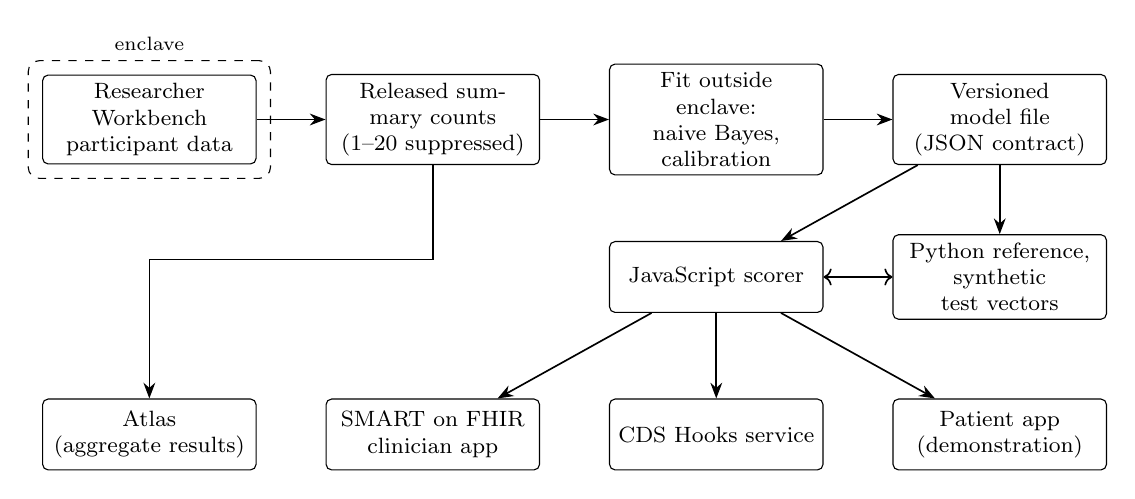
\begin{tikzpicture}[font=\footnotesize,
  box/.style={draw, rounded corners=2pt, align=center, minimum height=9mm, inner sep=3pt, text width=25mm},
  zone/.style={draw, dashed, rounded corners=4pt, inner sep=5pt},
  arr/.style={-{Stealth[length=2mm]}, semithick}]
\node[box] (wb) at (0,0) {Researcher Workbench\\participant data};
\node[box] (agg) at (3.6,0) {Released summary counts\\(1--20 suppressed)};
\node[box] (fit) at (7.2,0) {Fit outside enclave:\\naive Bayes, calibration};
\node[box] (json) at (10.8,0) {Versioned model file\\(JSON contract)};
\node[box] (js) at (7.2,-2) {JavaScript scorer};
\node[box] (ref) at (10.8,-2) {Python reference,\\synthetic test vectors};
\node[box] (smart) at (3.6,-4) {SMART on FHIR\\clinician app};
\node[box] (cds) at (7.2,-4) {CDS Hooks service};
\node[box] (pat) at (10.8,-4) {Patient app\\(demonstration)};
\node[box] (atlas) at (0,-4) {Atlas\\(aggregate results)};
\draw[arr] (wb) -- (agg); \draw[arr] (agg) -- (fit); \draw[arr] (fit) -- (json);
\draw[arr] (json) -- (ref); \draw[arr] (json) -- (js);
\draw[arr, <->] (js) -- (ref);
\draw[arr] (js) -- (smart); \draw[arr] (js) -- (cds); \draw[arr] (js) -- (pat);
\draw[arr] (agg.south) |- ++(0,-1.2) -| (atlas.north);
\begin{scope}[on background layer]
\node[zone, fit=(wb), label={[font=\scriptsize]above:enclave}] {};
\end{scope}
\end{tikzpicture}
\end{document}
